% Capital Allocation III -- how estimation error moves the optimizer, which input does it, and when the optimizer still wins.
% Figures and every number quoted here come from capital_allocation_figures.py
% Companion notebook: chapters/Finance/L13_CapitalAllocationIII_v2_AI.ipynb (parts 1-2 in class, the challenge is homework)
% The challenge answers (the alpha control, the covariance shrinkage intensity on the six factors, live shrinkage) and the Assignment 5
% answers must not appear here: this PDF is public. So no factor grid, and no out-of-sample race on the 49 industries.
\documentclass[aspectratio=169,10pt]{beamer}
\usetheme{default}
\usecolortheme{default}

\usepackage{graphicx}
\usepackage{adjustbox}
\usepackage{amsmath}
\usepackage{amssymb}
\usepackage{booktabs}
\usepackage{array}
\usepackage{tikz}
\usetikzlibrary{arrows.meta,positioning,calc,decorations.pathreplacing}
\usepackage{appendixnumberbeamer}  % Exclude appendix from slide count

\setbeamertemplate{navigation symbols}{}
\setbeamertemplate{items}[circle]

% Footline: Author, Event (Year) on left; page/total on right
\setbeamertemplate{footline}{
  \hbox{%
    \begin{beamercolorbox}[wd=.5\paperwidth,ht=2.5ex,dp=1ex,left]{author in head/foot}%
      \hspace*{2ex}\insertshortauthor, \insertshortinstitute\ (\insertdate)
    \end{beamercolorbox}%
    \begin{beamercolorbox}[wd=.5\paperwidth,ht=2.5ex,dp=1ex,right]{date in head/foot}%
      \insertframenumber/\inserttotalframenumber\hspace*{2ex}
    \end{beamercolorbox}%
  }
}

% Highlight boxes
\setbeamercolor{box1}{bg=red!12,fg=black}

% A poll option: {colour}{letter and choice}
\newcommand{\pollbox}[2]{\tikz\node[draw=#1!65!black, fill=#1!10, rounded corners=4pt, minimum width=3.7cm,
                                   minimum height=1.0cm, align=center, font=\normalsize]{#2};}
\newcolumntype{P}[1]{>{\raggedright\arraybackslash}p{#1}}

\title{Capital Allocation III}
\subtitle{When you have to estimate the inputs}
\author[A. Moreira]{Alan Moreira}
\institute[Data-Driven Investing]{NYU Stern --- Data-Driven Investing}
\date{Fall 2026}

\begin{document}

%------------------------------------------------------------------ 1
\begin{frame}
\titlepage
\end{frame}

\begin{frame}{Today}
\vskip 6pt
\begin{columns}[t]
\begin{column}{0.46\textwidth}
\textbf{In the slides}
\vskip 6pt
\begin{itemize}
\item Why estimation error makes the optimizer swing
\vskip 6pt
\item Which input does the damage: means, volatilities or correlations
\vskip 6pt
\item When the optimizer still wins, and shrinkage as the way in between
\end{itemize}
\end{column}
\begin{column}{0.50\textwidth}
\textbf{In the notebook, you will}
\vskip 6pt
\begin{itemize}
\item Race mean-variance against 1/N, and check which months went into each estimate
\vskip 6pt
\item Run six rules through the race
\vskip 6pt
\item Bootstrap the weights, one input at a time
\end{itemize}
\end{column}
\end{columns}
\vskip 16pt
\begin{beamercolorbox}[rounded=true,sep=7pt,center]{box1}
\textbf{Homework:} audit the book you built last class
\end{beamercolorbox}
\end{frame}

%================================================================== THE AMPLIFIER
%------------------------------------------------------------------ 2
\begin{frame}{In sample, the optimizer always wins}
\vskip 4pt
\begin{center}
\renewcommand{\arraystretch}{1.35}
\begin{tabular}{lc}
\toprule
six factors, 1980--2026 & Sharpe ratio, in sample \\
\midrule
mean-variance, $\Sigma^{-1}\mu$ & \textcolor{red}{1.17} \\
1/N & 1.03 \\
the best single factor (the market) & 0.57 \\
\bottomrule
\end{tabular}
\end{center}
\vskip 8pt
\begin{itemize}
\item It had to win. $\Sigma^{-1}\mu$ \emph{is} the maximum in this sample. That is algebra, not evidence.
\vskip 6pt
\item The real question: what does the formula do with inputs that are slightly wrong?
\end{itemize}
\vskip 10pt
\begin{beamercolorbox}[rounded=true,sep=7pt,center]{box1}
Optimization is in-sample fitting, and everything from \emph{Backtesting} applies to it
\end{beamercolorbox}
\end{frame}

%------------------------------------------------------------------ 3
\begin{frame}[label=amp]{A small error in the means does not stay small}
\[ W^{\star} = \tfrac{1}{\gamma}\,\Sigma^{-1}\mu \qquad\Longrightarrow\qquad \Delta W = \tfrac{1}{\gamma}\,\Sigma^{-1}\,\Delta\mu \]
\begin{center}
The error is multiplied by the inverse of the covariance matrix.
\end{center}
\vskip 2pt
Two assets, same volatility, weights adding to one:
\[ w_{1} \;=\; \frac{1}{2} \;+\; \frac{\text{gap}}{4 \times \text{average mean}} \times \textcolor{red}{\frac{1+\rho}{1-\rho}} \]
\begin{center}
\renewcommand{\arraystretch}{1.2}
\begin{tabular}{lccccc}
\toprule
correlation $\rho$ & 0 & 0.5 & 0.8 & 0.9 & 0.95 \\
\midrule
amplifier $(1+\rho)/(1-\rho)$ & 1 & 3 & 9 & \textcolor{red}{19} & 39 \\
weight on asset 1, 1pp gap, average mean 8\% & 53\% & 59\% & 78\% & \textcolor{red}{109\%} & 172\% \\
\bottomrule
\end{tabular}
\end{center}
\vskip 2pt
\hfill \hyperlink{appendix_two}{\beamerbutton{Derivation}}
\end{frame}

%------------------------------------------------------------------ 4
\begin{frame}{One percentage point, four different portfolios}
\begin{columns}[c]
\begin{column}{0.64\textwidth}
\adjustbox{max width=\textwidth, max height=0.76\textheight}{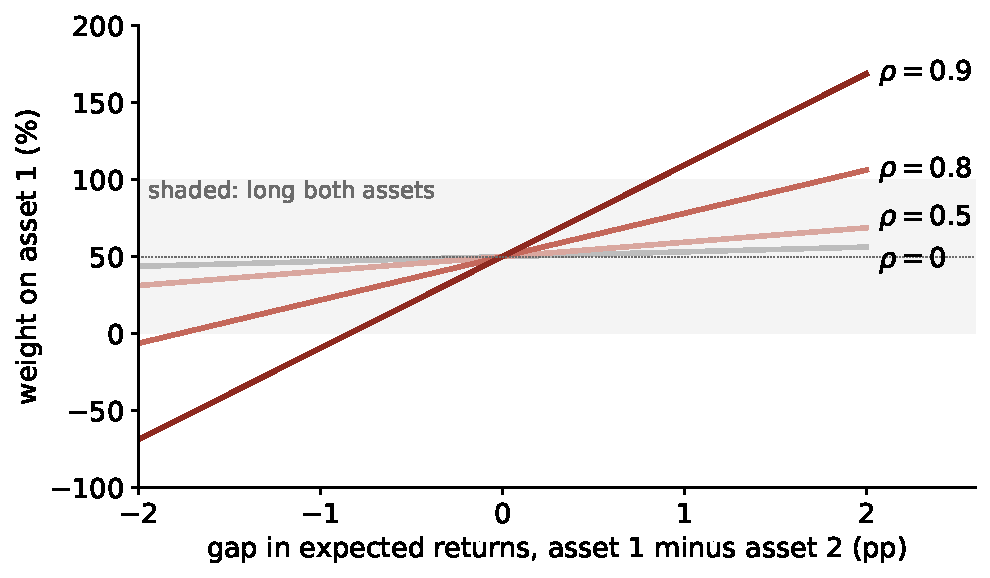
\includegraphics{figures/ca_amplifier.pdf}}
\end{column}
\begin{column}{0.34\textwidth}
\begin{itemize}
\item Zero correlation: a 1pp gap barely matters
\vskip 8pt
\item At $\rho=0.9$: 50/50 becomes \textcolor{red}{109/$-$9}
\vskip 8pt
\item Two good assets, and it shorts one
\vskip 8pt
\item Nobody can tell a 1pp gap in expected returns from zero
\end{itemize}
\end{column}
\end{columns}
\end{frame}

%------------------------------------------------------------------ 5
\begin{frame}{Why: correlation makes the spread look almost riskless}
\begin{columns}[c]
\begin{column}{0.50\textwidth}
\adjustbox{max width=\textwidth, max height=0.80\textheight}{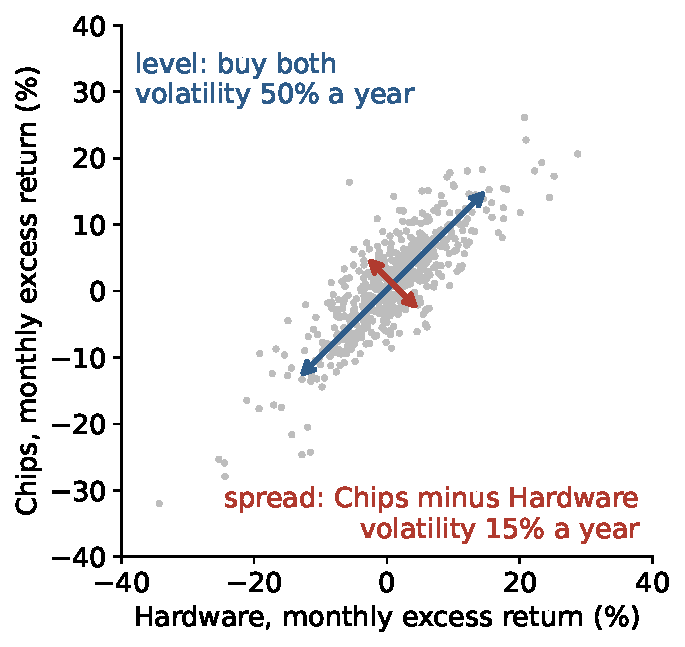
\includegraphics{figures/ca_pair_scatter.pdf}}
\end{column}
\begin{column}{0.48\textwidth}
Any pair is two bets: a \textcolor{blue}{level} and a \textcolor{red}{spread}.
\vskip 8pt
\[ \frac{\operatorname{Var}(\text{level})}{\operatorname{Var}(\text{spread})} = \frac{1+\rho}{1-\rho} = \frac{50\%^{2}}{15\%^{2}} = 11 \]
\vskip 4pt
\begin{itemize}
\item The optimizer sizes every bet by mean over variance
\vskip 6pt
\item The spread has a tiny variance, so a tiny gap earns a huge position
\vskip 6pt
\item The amplifier is that ratio of variances
\end{itemize}
\end{column}
\end{columns}
\end{frame}

%------------------------------------------------------------------ 6
\begin{frame}{A real pair: Hardware and Chips, $\rho = 0.84$}
\begin{columns}[c]
\begin{column}{0.60\textwidth}
\adjustbox{max width=\textwidth, max height=0.72\textheight}{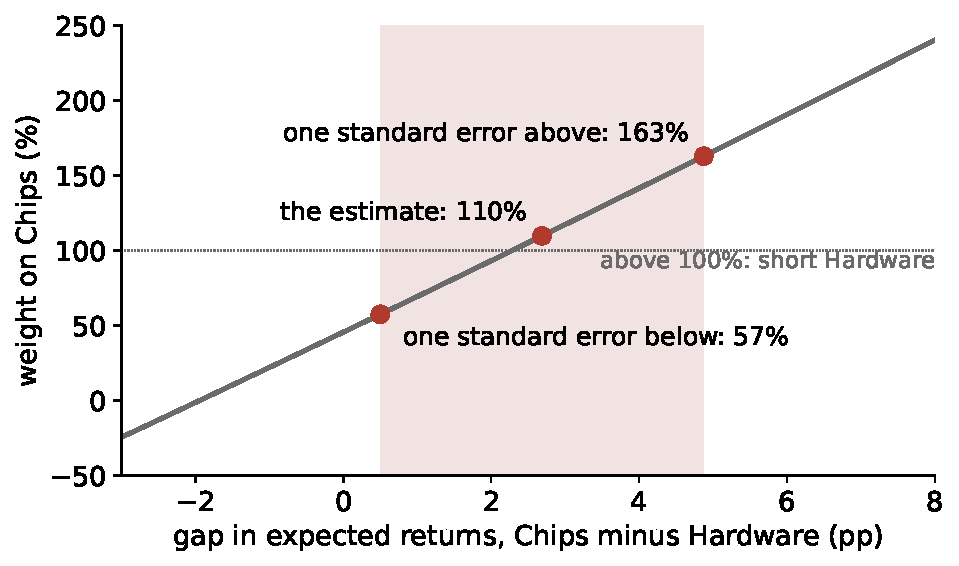
\includegraphics{figures/ca_pair_weights.pdf}}
\end{column}
\begin{column}{0.38\textwidth}
\renewcommand{\arraystretch}{1.2}
\begin{tabular}{lc}
\toprule
1980--2026 & mean $\pm$ s.e. \\
\midrule
Hardware & 10.6\% $\pm$ 3.8\% \\
Chips & 13.3\% $\pm$ 3.9\% \\
gap & \textcolor{red}{2.7\% $\pm$ 2.2\%} \\
\bottomrule
\end{tabular}
\vskip 10pt
\begin{itemize}
\item 46 years, and the gap is not distinguishable from zero
\vskip 6pt
\item One standard error is the difference between \textcolor{red}{57\%} and \textcolor{red}{163\%} in Chips
\vskip 6pt
\item At the estimate it shorts Hardware, a sector with a Sharpe ratio of 0.41
\end{itemize}
\end{column}
\end{columns}
\end{frame}

%------------------------------------------------------------------ 7
\begin{frame}{Same truth, same 46 years, three correlations}
\begin{center}
\adjustbox{max width=\textwidth, max height=0.44\textheight}{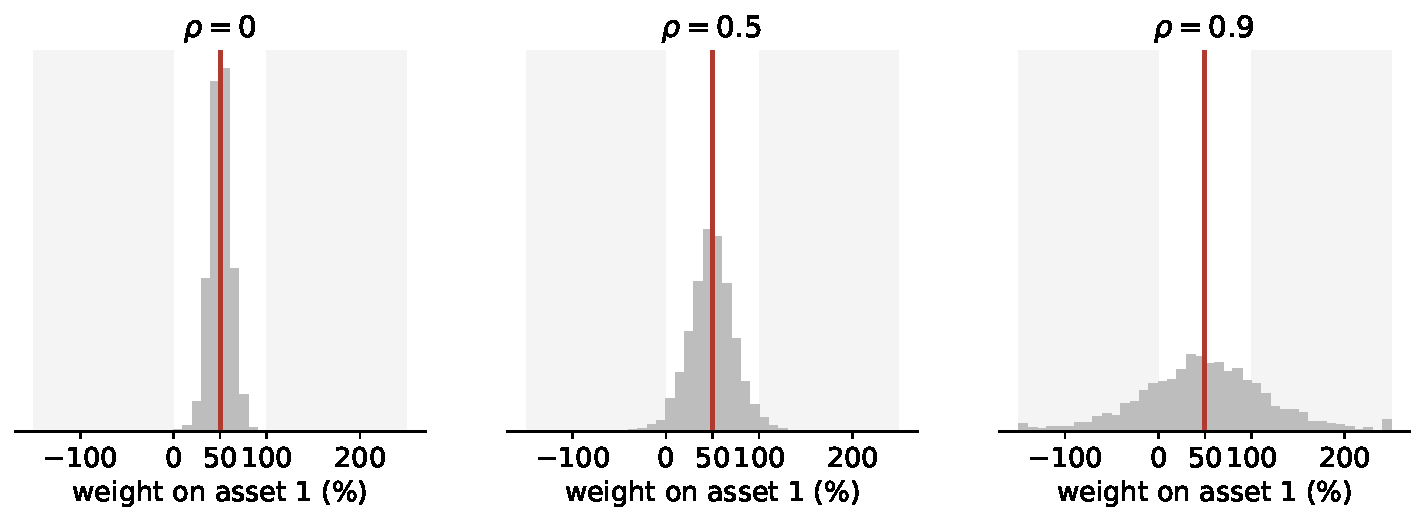
\includegraphics{figures/ca_same_truth.pdf}}
\end{center}
\vskip 2pt
{\small Both assets: true mean 8\%, volatility 16\%. The right answer is always 50/50 (red). Shaded: a short position.}
\vskip 6pt
\begin{itemize}
\item 90\% of histories: 32\% to 69\% at $\rho=0$; \textcolor{red}{$-65\%$ to 165\%} at $\rho=0.9$, short in 44\% of them
\vskip 5pt
\item In fairness, correlation also helps: the gap is better estimated, its error falls with $\sqrt{1-\rho}$
\vskip 5pt
\item But the amplifier grows with $1/(1-\rho)$. Net, the weight's error grows with $(1+\rho)/\sqrt{1-\rho}$
\end{itemize}
\end{frame}

%================================================================== WHICH INPUT
%------------------------------------------------------------------ 8
\begin{frame}{The formula has three inputs, each with a standard error}
\vskip 4pt
\begin{center}
\renewcommand{\arraystretch}{1.45}
\begin{tabular}{lccc}
\toprule
input & standard error & example, per year & error, \% of estimate \\
\midrule
expected return & $\sigma/\sqrt{T}$ & HML mean: 2.8\% $\pm$ 1.6\% & \textcolor{red}{57\%} \\
volatility & $\sigma/\sqrt{2T}$ & HML volatility: 10.9\% $\pm$ 0.3\% & 3\% \\
correlation & $(1-\rho^{2})/\sqrt{T}$ & market and HML: $-0.21 \pm 0.04$ & 19\% \\
\bottomrule
\end{tabular}
\end{center}
\vskip 10pt
\begin{itemize}
\item $T$ is the number of observations in the time series: here 558 months. $\sigma$ is the volatility per observation.
\vskip 6pt
\item Daily data raises $T$, and shrinks the error on volatilities and correlations. The error on a yearly mean does not move: only more years help.
\vskip 6pt
\item With $N$ assets: $N$ means, $N$ volatilities, $N(N-1)/2$ correlations
\vskip 6pt
\item What matters is not the size of the error, but what it does to the portfolio.
\end{itemize}
\end{frame}

%------------------------------------------------------------------ 9
\begin{frame}{Poll}
\vskip 14pt
\begin{center}
{\large Six factors, 46 years of data. You re-estimate one kind of input\\[4pt] and leave the other two alone.}
\vskip 18pt
Which one moves your portfolio the most?
\vskip 18pt
\pollbox{red}{\textbf{A}\ \ the means} \hfill
\pollbox{gray}{\textbf{B}\ \ the volatilities} \hfill
\pollbox{blue}{\textbf{C}\ \ the correlations}
\end{center}
\end{frame}

%------------------------------------------------------------------ 10
\begin{frame}{Exercise 1: move one number by one standard error}
\begin{center}
\adjustbox{max width=\textwidth, max height=0.56\textheight}{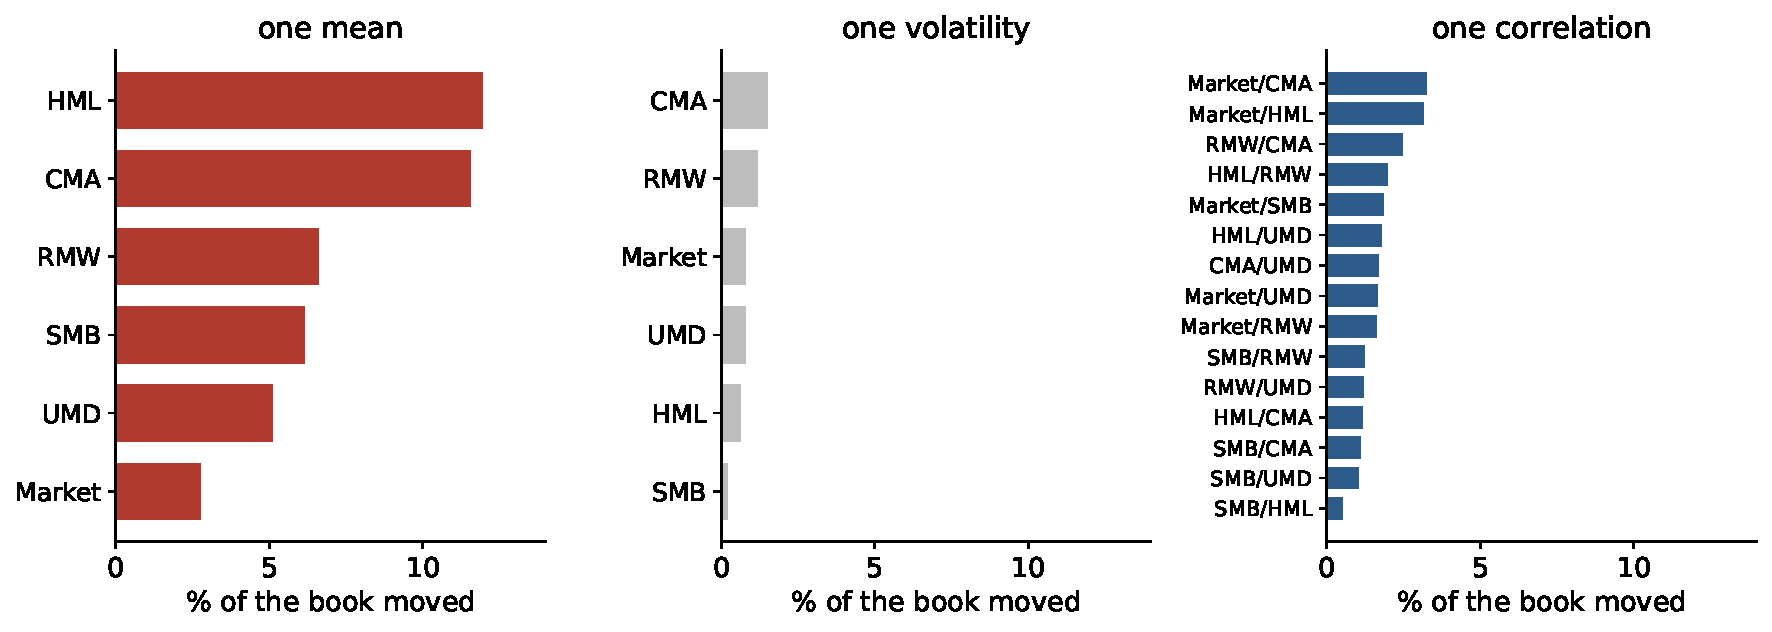
\includegraphics{figures/ca_one_se.pdf}}
\end{center}
\vskip 2pt
\begin{itemize}
\item Every bar: change one input, hold the other 26 fixed, count how much of the book changes hands
\vskip 5pt
\item Largest move: a mean \textcolor{red}{12\%}, a correlation 3.3\%, a volatility 1.5\%
\vskip 5pt
\item But standard errors do not arrive one at a time, and there are 15 correlations
\end{itemize}
\end{frame}

%------------------------------------------------------------------ 11
\begin{frame}[label=boot_back]{Exercise 2: move them all, as history would}
\begin{center}
\adjustbox{max width=\textwidth, max height=0.50\textheight}{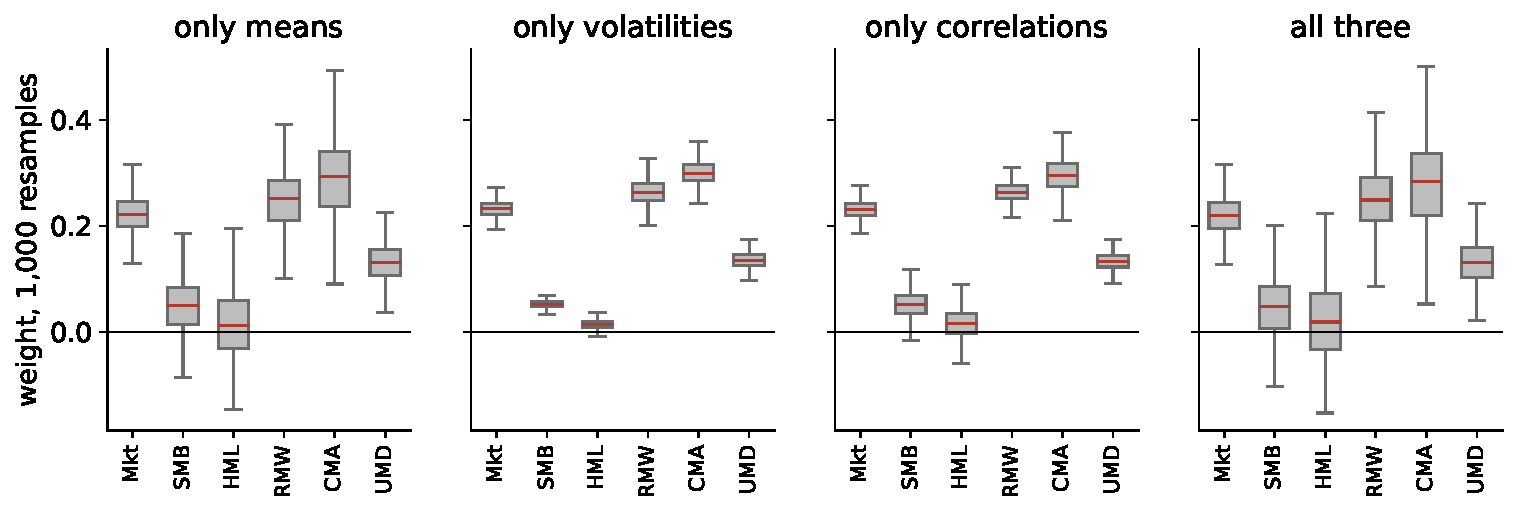
\includegraphics{figures/ca_boot_inputs.pdf}}
\end{center}
\vskip 2pt
\begin{itemize}
\item Resample the 558 months, 1,000 times. Each draw gives new means, volatilities and correlations.
\vskip 5pt
\item Feed in one kind at a time, the other two at their full-sample values. Then all three.
\vskip 5pt
\item Variance of the weights: \textcolor{red}{79\% means}, 14\% correlations, 7\% volatilities
\end{itemize}
\vskip 2pt
\hfill \hyperlink{appendix_boot}{\beamerbutton{The bootstrap, in a picture}}
\end{frame}

%------------------------------------------------------------------ 12
\begin{frame}{Who is to blame depends on what you hold}
\vskip 2pt
\begin{center}
\renewcommand{\arraystretch}{1.3}
\begin{tabular}{lccc@{\hskip 16pt}ccc@{\hskip 16pt}c}
\toprule
 & \multicolumn{3}{c}{variance of the weights} & \multicolumn{3}{c}{Sharpe ratio lost} & Sharpe lost, \\
 & means & vols & corrs & means & vols & corrs & ten years of data \\
\midrule
six factors & 79\% & 7\% & 14\% & 3.8\% & 0.5\% & 0.6\% & 18\% \\
eight sectors & \textcolor{red}{88\%} & 6\% & 6\% & \textcolor{red}{10.1\%} & 0.4\% & 0.5\% & 34\% \\
five asset classes & \textcolor{red}{96\%} & 2\% & 2\% & \textcolor{red}{10.3\%} & 0.3\% & 0.2\% & 36\% \\
29 long-shorts & 35\% & 8\% & \textcolor{red}{57\%} & 5.3\% & 1.2\% & \textcolor{red}{8.8\%} & 27\% \\
\bottomrule
\end{tabular}
\end{center}
\vskip 8pt
\begin{itemize}
\item Volatilities are never the problem
\vskip 5pt
\item A few assets: the means. 29 strategies have 406 correlations, some near 0.97: they overtake the means.
\vskip 5pt
\item Sharpe lost as a share of the best, using all the data unless stated
\end{itemize}
\vskip 6pt
{\small Careful: this world takes the sample means as the truth. So it overstates how different the assets are. We come back to this.}
\end{frame}

%================================================================== THE MENU
%------------------------------------------------------------------ 13
\begin{frame}{Each rule replaces an estimate with a constant}
\vskip 2pt
\begin{center}
\renewcommand{\arraystretch}{1.3}
\adjustbox{max width=\textwidth}{\begin{tabular}{llllll}
\toprule
rule & weights & the constant & \multicolumn{3}{c}{still estimates} \\
\midrule
mean-variance & $\Sigma^{-1}\mu$ & none & \textcolor{red}{means} & vols & corrs \\
no correlations & $\mu_{i}/\sigma_{i}^{2}$ & every correlation is zero & \textcolor{red}{means} & vols & \\
same Sharpe & $\Sigma^{-1}\sigma$ & every Sharpe ratio is equal & & vols & corrs \\
same mean & $\Sigma^{-1}\mathbf{1}$ & every expected return is equal & & vols & corrs \\
risk parity & $1/\sigma_{i}$ & same Sharpe, no correlations & & vols & \\
1/N & $1/N$ & same Sharpe, no correlations, same vol & & & \\
\bottomrule
\end{tabular}}
\end{center}
\vskip 10pt
\begin{itemize}
\item ``Same mean'' is minimum-variance. Risk parity is $w_{i}\sigma_{i} \propto AR_{i}$ from \emph{Capital Allocation II}, with the ratios set equal.
\vskip 6pt
\item None of these is simply better. Each is a claim about your assets.
\end{itemize}
\end{frame}

%------------------------------------------------------------------ 14
\begin{frame}{Change the rule, change what you are exposed to}
\begin{center}
\adjustbox{max width=\textwidth, max height=0.52\textheight}{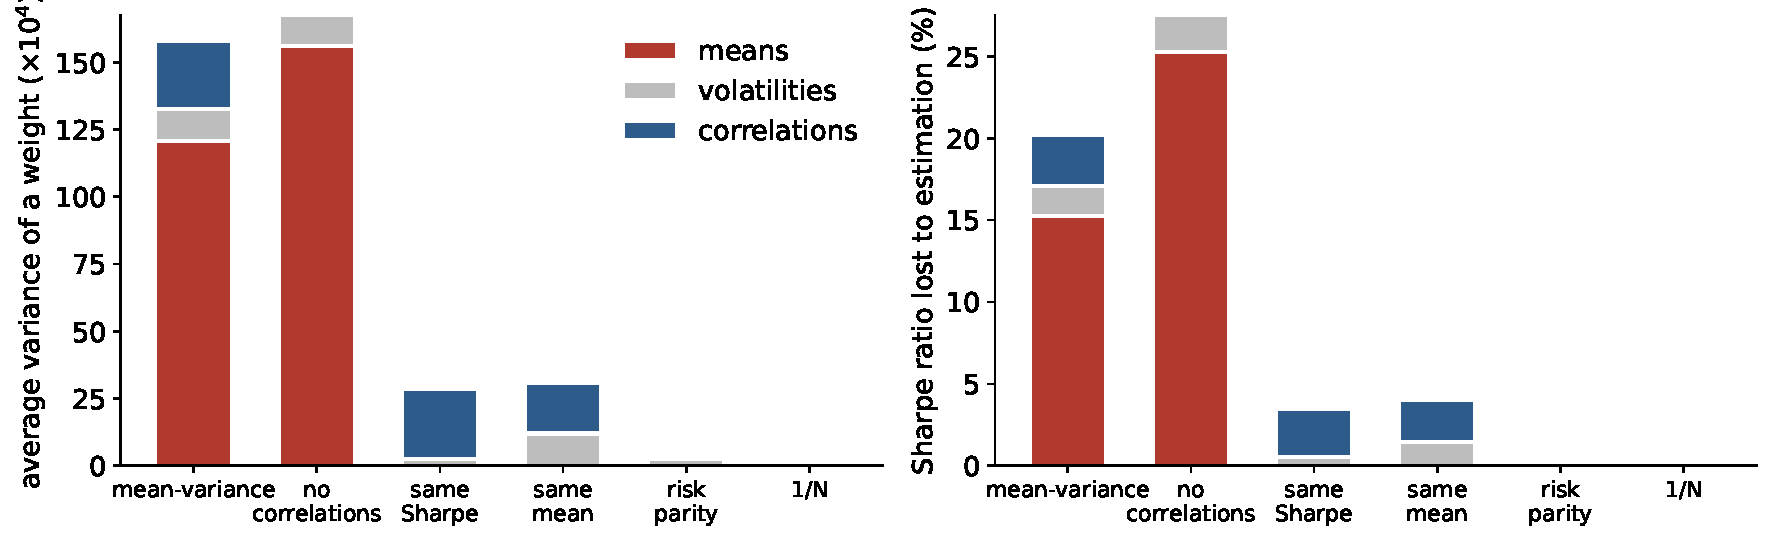
\includegraphics{figures/ca_boot_rules.pdf}}
\end{center}
\vskip 2pt
{\small Six factors, each history ten years long. Each input moved separately.}
\vskip 4pt
\begin{itemize}
\item Stop estimating the means and the exposure collapses: Sharpe lost \textcolor{red}{18\% to 3\%}. With all 46 years: 5\% to 1\%.
\vskip 4pt
\item Ignoring correlations does not help. The noise in the means is still there, with no hedge against it.
\vskip 4pt
\item 1/N has no exposure at all. Is that free? Only if its constant is right.
\end{itemize}
\end{frame}

%------------------------------------------------------------------ 15
\begin{frame}{Now: the notebook}
\vskip 2pt
\begin{beamercolorbox}[rounded=true,sep=7pt,center]{box1}
\textbf{Notebook: Capital Allocation III} \ --- \ the rules, out of sample
\end{beamercolorbox}
\vskip 10pt
\begin{enumerate}
\item \textbf{``Is this out of sample?''} Race mean-variance against 1/N with AI, then read which months went into each estimate.
\vskip 5pt
\item \textbf{The menu.} The six rules, the race, and the bootstrap one input at a time.
\end{enumerate}
\vskip 8pt
{\small \textbf{Bring back:} which rule won the race, and would you bet that it wins on \emph{any} set of assets? \\[2pt]
Stop at \textbf{Back to the slides}; the challenge after it is homework.}
\end{frame}

%================================================================== THE RACE
%------------------------------------------------------------------ 16
\begin{frame}{1/N won. One index would have reversed it.}
\vskip 2pt
\begin{center}
\renewcommand{\arraystretch}{1.25}
\begin{tabular}{lc}
\toprule
six factors, expanding window, ten-year burn-in & Sharpe ratio, out of sample \\
\midrule
1/N & \textcolor{red}{0.92} \\
mean-variance & 0.83 \\
same Sharpe & 0.83 \\
same mean & 0.77 \\
risk parity & 0.76 \\
\midrule
mean-variance, estimate includes the month it earns & \textcolor{red}{1.03} \\
\bottomrule
\end{tabular}
\end{center}
\vskip 6pt
\begin{itemize}
\item DeMiguel, Garlappi and Uppal (2009): the formula loses to dividing by the number of assets
\vskip 4pt
\item Written with \texttt{F.iloc[:t+1]} instead of \texttt{F.iloc[:t]}, the conclusion flips. Your AI may not warn you.
\vskip 4pt
\item The gap is $0.09 \pm 0.10$. It is not a law of nature, so run the same race on other assets.
\end{itemize}
\end{frame}

%------------------------------------------------------------------ 17
\begin{frame}{Same race, other assets: the winner changes}
\vskip 4pt
\begin{center}
\renewcommand{\arraystretch}{1.4}
\adjustbox{max width=\textwidth}{\begin{tabular}{llccc}
\toprule
ten-year burn-in, before costs & period & mean-variance & 1/N & 1/N minus mean-variance \\
\midrule
29 long-shorts & 1980--2000 & \textcolor{red}{2.24} & 0.98 & $-1.25 \pm 0.39$ \\
six factors & 1980--2026 & 0.83 & 0.92 & $+0.09 \pm 0.10$ \\
eight sectors & 1980--2026 & 0.46 & \textcolor{red}{0.64} & $+0.18 \pm 0.17$ \\
five asset classes & 1963--2016 & 0.39 & \textcolor{red}{0.50} & $+0.11 \pm 0.13$ \\
\bottomrule
\end{tabular}}
\end{center}
\vskip 12pt
\begin{itemize}
\item ``1/N beats the optimizer'' is not a result. It is a result about particular assets.
\vskip 6pt
\item So what do the assets have to look like?
\end{itemize}
\vskip 8pt
{\small Careful with the 29: they were chosen later because they worked in this very period, and the optimizer trades them heavily. Treat 2.24 as an upper bound. The gaps in the last three rows are within about one standard error.}
\end{frame}

%------------------------------------------------------------------ 18
\begin{frame}[label=formula]{The race, in one formula}
The optimizer sees $N$ independent bets, and from \emph{Capital Allocation II} their Sharpe ratios add in squares.
\vskip 6pt
\begin{itemize}
\item Each bet also carries a fake Sharpe ratio of about $\pm 1/\sqrt{Y}$, with $Y$ the years of data and Sharpe ratios per year
\vskip 4pt
\item The squares of the fakes add up too: $N/Y$
\end{itemize}
\[ \underbrace{SR^{2}_{\text{in sample}}}_{\text{what you see}} \;\approx\; \underbrace{SR^{2}}_{\text{real differences}} + \underbrace{N/Y}_{\text{estimation error}}
\qquad\Longrightarrow\qquad
\frac{SR_{\text{you earn}}}{SR} \;\approx\; \frac{1}{\sqrt{1 + \dfrac{N}{Y\,SR^{2}}}} \]
\vskip 4pt
\begin{beamercolorbox}[rounded=true,sep=7pt,center]{box1}
A race between how different your assets really are and how noisy your estimates are
\end{beamercolorbox}
\vskip 6pt
\begin{itemize}
\item Correlation enters through $SR$: for the same assets, high $\rho$ means a lower $SR$, so noise matters more
\end{itemize}
\hfill \hyperlink{appendix_formula}{\beamerbutton{Derivation}}
\end{frame}

%------------------------------------------------------------------ 19
\begin{frame}{The optimizer learns, 1/N does not, and the crossing moves}
\begin{center}
\adjustbox{max width=\textwidth, max height=0.50\textheight}{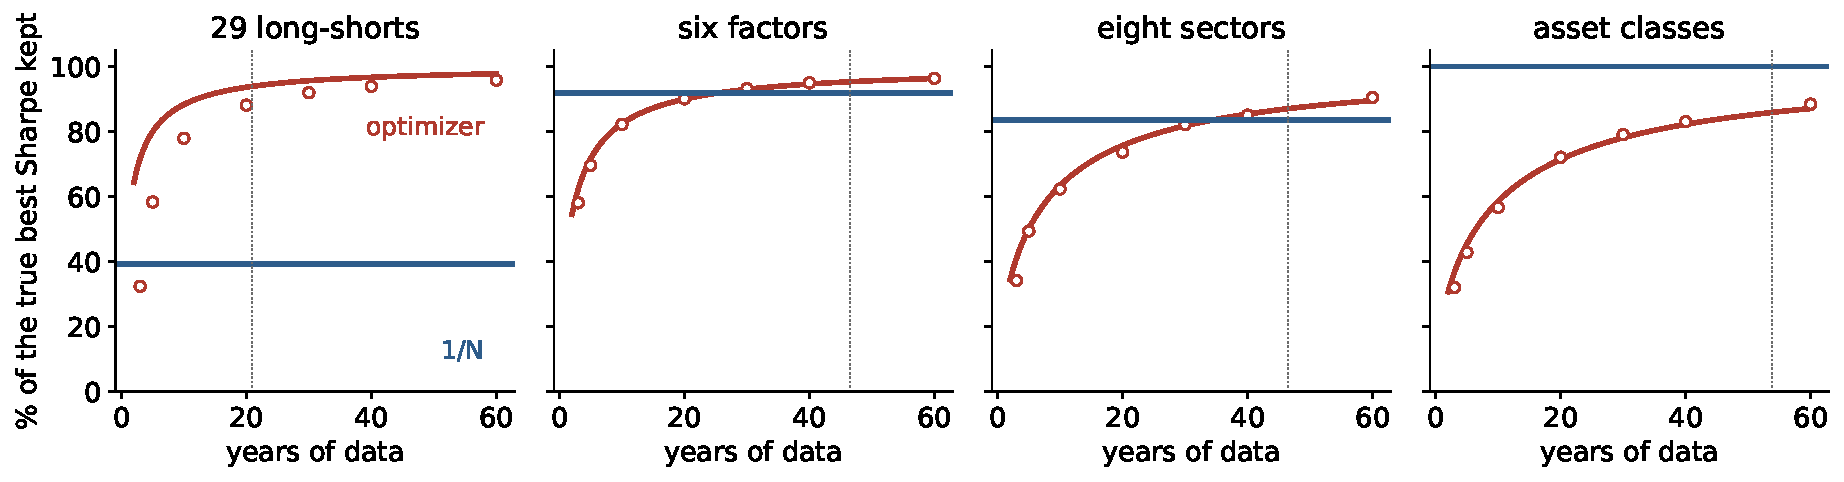
\includegraphics{figures/ca_race.pdf}}
\end{center}
\vskip 2pt
{\small A world we control, built from each asset set. Line: the formula. Dots: simulation, estimating everything. Dotted: the years we actually have.}
\vskip 6pt
\begin{itemize}
\item 29 long-shorts: differences so large the optimizer wins almost at once
\vskip 4pt
\item Factors and sectors: it takes decades. Asset classes: 1/N is already about as good as it gets.
\end{itemize}
\vskip 2pt
\hfill \hyperlink{appendix_world}{\beamerbutton{The simulated world}}
\end{frame}

%------------------------------------------------------------------ 20
\begin{frame}{Real differences, or noise?}
\vskip 2pt
\begin{center}
\renewcommand{\arraystretch}{1.3}
\begin{tabular}{lcccccc}
\toprule
 & \multicolumn{2}{c}{Sharpe ratio, in sample} & \multicolumn{2}{c}{extra $SR^{2}$ beyond 1/N} & noise & years to \\
 & 1/N & best & seen & noise, $(N-1)/Y$ & share & beat 1/N \\
\midrule
29 long-shorts & 1.25 & 3.40 & 10.01 & 1.34 & \textcolor{red}{13\%} & \textcolor{red}{under 1} \\
six factors & 1.03 & 1.17 & 0.31 & 0.11 & 35\% & 25 \\
eight sectors & 0.61 & 0.83 & 0.31 & 0.15 & 48\% & 35 \\
five asset classes & 0.51 & 0.56 & 0.06 & 0.07 & \textcolor{red}{128\%} & \textcolor{red}{never} \\
\bottomrule
\end{tabular}
\end{center}
\vskip 8pt
\begin{itemize}
\item It lines up with the race, whose average window was 28 years: under 1 year is an easy win, 25 is a coin flip, 35 is a loss
\vskip 5pt
\item Asset classes: all of the extra Sharpe ratio you see is what noise alone would produce
\end{itemize}
\vskip 6pt
\begin{beamercolorbox}[rounded=true,sep=7pt,center]{box1}
Similar assets: error dominates, assume a constant. Very different assets: a constant throws the signal away.
\end{beamercolorbox}
\end{frame}

%------------------------------------------------------------------ 21
\begin{frame}{Which constant? It has to fit the assets too}
\vskip 2pt
\begin{center}
\renewcommand{\arraystretch}{1.25}
\adjustbox{max width=\textwidth}{\begin{tabular}{lcc@{\hskip 16pt}cccc}
\toprule
 & \multicolumn{2}{c}{range, in sample} & \multicolumn{4}{c}{Sharpe ratio, out of sample} \\
 & means & Sharpes & same mean & same Sharpe & mean-variance & 1/N \\
\midrule
five asset classes & 2.5\% to 8.1\% & 0.25 to 0.41 & 0.45 & \textcolor{red}{0.55} & 0.39 & 0.50 \\
eight sectors & 7.3\% to 11.9\% & 0.30 to 0.76 & 0.44 & \textcolor{red}{0.71} & 0.46 & 0.64 \\
six factors & 0.7\% to 8.9\% & 0.07 to 0.57 & 0.77 & 0.83 & 0.83 & 0.92 \\
29 long-shorts & $-6.4\%$ to 19.9\% & $-0.57$ to 1.36 & 1.07 & 1.08 & \textcolor{red}{2.24} & 0.98 \\
\bottomrule
\end{tabular}}
\end{center}
\vskip 8pt
\begin{itemize}
\item Same mean on stocks and bonds is ill-advised: it puts \textcolor{red}{82\%} in foreign government bonds, for having low volatility
\vskip 5pt
\item Bonds and emerging markets do not earn the same return. They may earn about the same Sharpe ratio.
\vskip 5pt
\item Sectors have similar means, yet same mean does not rescue them: $0.44$ against $0.46$. Same Sharpe does.
\vskip 5pt
\item On the 29, either constant throws away half the Sharpe ratio. Those assets really are different.
\end{itemize}
\end{frame}

%================================================================== SHRINKAGE
%------------------------------------------------------------------ 22
\begin{frame}{Shrinkage: the same choice, made continuous}
\begin{columns}[c]
\begin{column}{0.50\textwidth}
\begin{center}
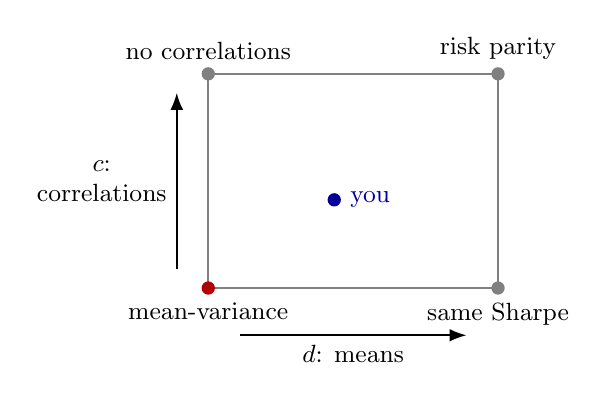
\begin{tikzpicture}[scale=0.8]
\draw[line width=0.8pt, gray] (0,0) rectangle (4.6,3.4);
\fill[red!70!black] (0,0) circle (3pt);
\fill[gray] (4.6,0) circle (3pt);
\fill[gray] (0,3.4) circle (3pt);
\fill[gray] (4.6,3.4) circle (3pt);
\fill[blue!60!black] (2.0,1.4) circle (3pt);
\node[below, align=center, font=\small] at (0,-0.08) {mean-variance};
\node[below, align=center, font=\small] at (4.6,-0.08) {same Sharpe};
\node[above, align=center, font=\small] at (0,3.48) {no correlations};
\node[above, align=center, font=\small] at (4.6,3.48) {risk parity};
\node[right, font=\small, blue!60!black] at (2.1,1.4) {you};
\draw[-{Latex}, line width=0.7pt] (0.5,-0.75) -- node[below, font=\small]{$d$: means} (4.1,-0.75);
\draw[-{Latex}, line width=0.7pt] (-0.5,0.3) -- node[left, align=center, font=\small]{$c$:\\correlations} (-0.5,3.1);
\end{tikzpicture}
\end{center}
\end{column}
\begin{column}{0.46\textwidth}
One dial per input:
\[ s_{i}(d) = (1-d)\,\hat s_{i} + d\,\bar s \]
\[ R(c) = (1-c)\,\hat R + c\,I \]
\begin{itemize}
\item The rules are the corners. Shrinkage lets you stand anywhere in between.
\vskip 6pt
\item Set all the volatilities equal too and risk parity becomes 1/N
\vskip 6pt
\item Long-only and position caps work the same way: a constraint is a prior
\end{itemize}
\end{column}
\end{columns}
\end{frame}

%------------------------------------------------------------------ 23
\begin{frame}{Same two dials, opposite answers}
\begin{center}
\adjustbox{max width=\textwidth, max height=0.56\textheight}{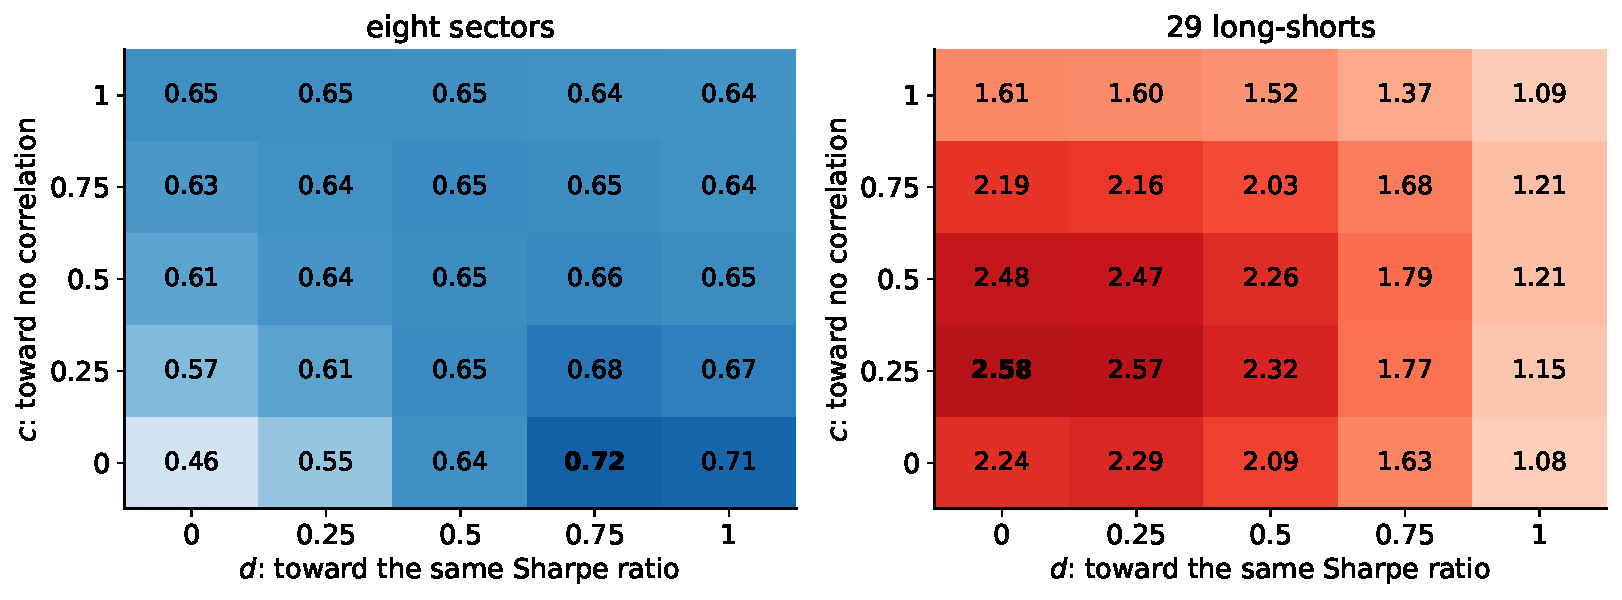
\includegraphics{figures/ca_dial_grid.pdf}}
\end{center}
\vskip 2pt
\begin{itemize}
\item Sectors: turn the means dial, $0.46 \to \textcolor{red}{0.72}$. Their means are mostly noise.
\vskip 5pt
\item The 29: leave the means, turn the correlations a little, $2.24 \to \textcolor{red}{2.58}$. Just as Exercise 2 said: 57\% of their weight variance came from correlations.
\vskip 5pt
\item Out of sample, before costs. Picking the best cell afterward is itself in-sample fitting.
\end{itemize}
\end{frame}

%------------------------------------------------------------------ 24
\begin{frame}{How far to turn the dial is the race again}
\begin{columns}[c]
\begin{column}{0.62\textwidth}
\adjustbox{max width=\textwidth, max height=0.72\textheight}{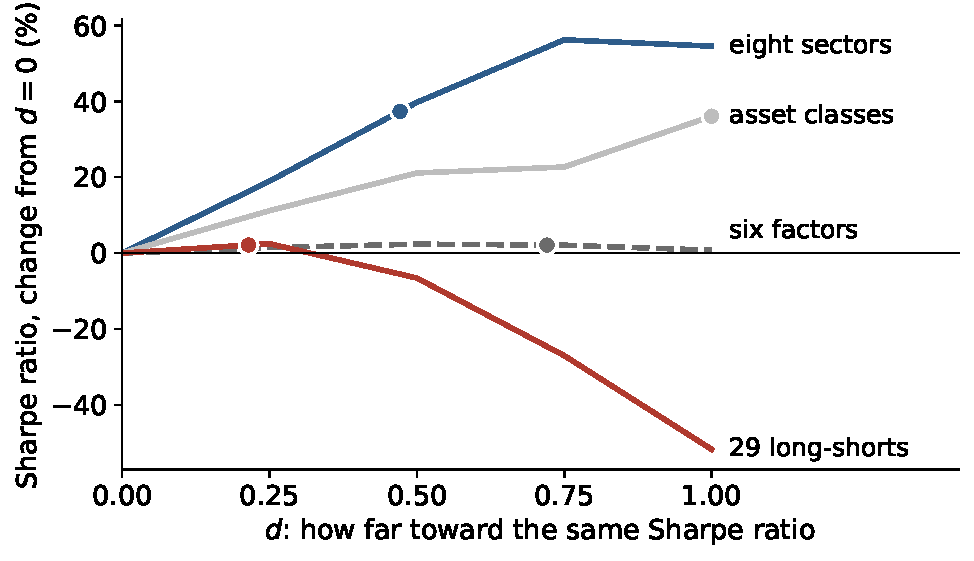
\includegraphics{figures/ca_dial_path.pdf}}
\end{column}
\begin{column}{0.36\textwidth}
\[ d \;\approx\; \frac{\text{noise}}{\text{dispersion you see}} \]
{\small in the Sharpe ratios across assets; the dots}
\vskip 8pt
\begin{itemize}
\item It can help or hurt: \textcolor{red}{$+56\%$} on sectors, \textcolor{red}{$-52\%$} on the 29
\vskip 6pt
\item The rule gets the direction and the rough size. On sectors it says 0.47, the best was 0.75.
\vskip 6pt
\item The logic of Black-Litterman: weigh the prior against the noise in the estimate
\end{itemize}
\end{column}
\end{columns}
\end{frame}

%------------------------------------------------------------------ 25
\begin{frame}{What to actually do}
\vskip 6pt
\begin{enumerate}
\item \textbf{Ask how different your assets really are.} Compare $SR^{2}$ with $N/Y$ before you trust a formula, or a rule of thumb.
\vskip 8pt
\item \textbf{Look at the correlations.} Above about 0.8, you are mostly trading a spread. Ask whether you believe the gap.
\vskip 8pt
\item \textbf{Use data on what data can teach}: volatilities first. Correlations too, unless $N$ is large.
\vskip 8pt
\item \textbf{Turn dials, do not pick sides.} Similar assets: near the constant. Very different assets: near the estimates.
\vskip 8pt
\item \textbf{Treat the dial as a parameter}: tune it without the future, test it, report once, and count costs.
\end{enumerate}
\end{frame}

%------------------------------------------------------------------ 26
\begin{frame}{Takeaways}
\begin{enumerate}
\item The formula multiplies input errors by $\Sigma^{-1}$. For two correlated assets the amplifier is $(1+\rho)/(1-\rho)$.
\vskip 4pt
\item In a small book the means do the damage. In a large one the correlations can take over. Volatilities never do.
\vskip 4pt
\item Each rule replaces an estimate with a constant, and is exposed only to what it still estimates.
\vskip 4pt
\item Whether that helps is a race: real differences, $SR^{2}$, against estimation error, $N/Y$.
\vskip 4pt
\item 1/N beats the optimizer on similar assets, and loses badly on very different ones.
\vskip 4pt
\item Shrinkage is the rules made continuous, and how far to go depends on the assets.
\end{enumerate}
\vskip 8pt
\begin{beamercolorbox}[rounded=true,sep=7pt]{box1}
\textbf{Homework: audit the book.} Throw the alphas away and see what happens, out of sample. Then find the right amount of shrinkage, and find out whether you could have known it.
\end{beamercolorbox}
\end{frame}

%================================================================== APPENDIX
\appendix
\begin{frame}
\begin{center}
{\Large Appendix}
\end{center}
\end{frame}

\begin{frame}[label=appendix_two]{A1: Two assets}
Same volatility $\sigma$, correlation $\rho$, means $\mu_{1} = \bar\mu + g/2$ and $\mu_{2} = \bar\mu - g/2$.
\[ \Sigma^{-1}\mu \;\propto\; \begin{pmatrix}1 & -\rho \\ -\rho & 1\end{pmatrix}\begin{pmatrix}\mu_{1} \\ \mu_{2}\end{pmatrix} \;=\; \begin{pmatrix}\mu_{1} - \rho \mu_{2} \\ \mu_{2} - \rho \mu_{1}\end{pmatrix} \]
\vskip 2pt
The two entries add to $2\bar\mu(1-\rho)$, and the first is $\bar\mu(1-\rho) + \tfrac{g}{2}(1+\rho)$. So
\[ w_{1} = \frac{1}{2} + \frac{g}{4\bar\mu}\cdot\frac{1+\rho}{1-\rho} \]
\begin{itemize}
\item Asset 2 is shorted when $\mu_{2}/\mu_{1} < \rho$. With different volatilities, the same test on Sharpe ratios.
\vskip 5pt
\item With $Y$ years of data, the error in $g$ is $\sigma\sqrt{2(1-\rho)/Y}$, so the error in $w_{1}$ is $\dfrac{1+\rho}{4\,(\bar\mu/\sigma)}\sqrt{\dfrac{2}{Y(1-\rho)}}$. With $\bar\mu/\sigma = 0.5$, $Y = 46$: 10\%, 22\%, 62\%.
\end{itemize}
\hfill \hyperlink{amp}{\beamerreturnbutton{Back}}
\end{frame}

\begin{frame}[label=appendix_formula]{A2: The formula for the race}
Whiten the assets: $z = \Sigma^{-1/2}\mu$, so $|z|^{2} = SR^{2}$. The estimate of $z$ is $z + u$, with $u$ noise of variance $1/Y$ in each of $N$ directions.
\vskip 6pt
\begin{itemize}
\item In sample you see $|z+u|^{2} \approx SR^{2} + N/Y$
\vskip 5pt
\item Your portfolio points along $z + u$. Under the truth it earns $\dfrac{z'(z+u)}{|z+u|} \approx \dfrac{SR^{2}}{\sqrt{SR^{2} + N/Y}}$
\vskip 5pt
\item Against 1/N, which keeps a share $q$ of the true best, the optimizer wins once $Y > \dfrac{N}{SR^{2}}\cdot\dfrac{q^{2}}{1-q^{2}}$
\vskip 5pt
\item This covers errors in the means only. Errors in $\Sigma$ add to it when $N$ is large relative to the data: see the dots for the 29.
\end{itemize}
\hfill \hyperlink{formula}{\beamerreturnbutton{Back}}
\end{frame}

\begin{frame}[label=appendix_world]{A3: The simulated world}
\begin{itemize}
\item \textbf{Covariances}: each asset set's sample $\Sigma$, with normal returns
\vskip 7pt
\item \textbf{1/N}: keeps its sample Sharpe ratio. No selection went into it, so it needs no correction.
\vskip 7pt
\item \textbf{The rest}: the extra $SR^{2}$ beyond 1/N, minus the $(N-1)/Y$ that noise alone would produce
\vskip 7pt
\item \textbf{Score}: the Sharpe ratio under the truth, over the true best. Mean of 300 histories.
\vskip 7pt
\item \textbf{The limit}: a stable world, correctly specified, and a noisy estimate of how much signal there is. Real markets move, so read the years as a lower bound.
\end{itemize}
\hfill \hyperlink{appendix_world_back}{\beamerreturnbutton{Back}}
\end{frame}

\begin{frame}[label=appendix_boot]{A4: The bootstrap, in a picture}
\begin{center}
\adjustbox{max width=\textwidth}{%
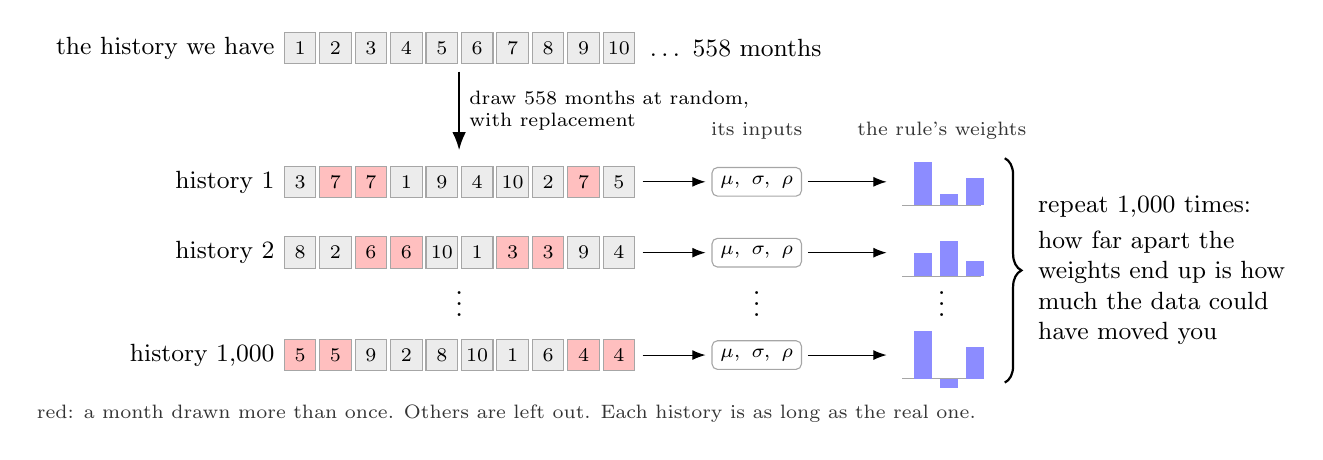
\begin{tikzpicture}[x=1cm, y=1cm, month/.style={draw=gray!70, minimum size=0.40cm, inner sep=0pt, font=\scriptsize}]
% the real history
\node[anchor=east, font=\small] at (2.20,4.6) {the history we have};
\node[month, fill=gray!15] at (2.40,4.6) {1};
\node[month, fill=gray!15] at (2.85,4.6) {2};
\node[month, fill=gray!15] at (3.30,4.6) {3};
\node[month, fill=gray!15] at (3.75,4.6) {4};
\node[month, fill=gray!15] at (4.20,4.6) {5};
\node[month, fill=gray!15] at (4.65,4.6) {6};
\node[month, fill=gray!15] at (5.10,4.6) {7};
\node[month, fill=gray!15] at (5.55,4.6) {8};
\node[month, fill=gray!15] at (6.00,4.6) {9};
\node[month, fill=gray!15] at (6.45,4.6) {10};
\node[anchor=west, font=\small] at (6.72,4.6) {$\dots$ 558 months};
\draw[-{Latex}, thick] (4.42,4.3) -- (4.42,3.3) node[midway, right, font=\scriptsize, align=left] {draw 558 months at random,\\ with replacement};
% column headers
\node[font=\scriptsize, gray!40!black] at (8.2,3.55) {its inputs};
\node[font=\scriptsize, gray!40!black] at (10.55,3.55) {the rule's weights};
% made-up histories
\node[anchor=east, font=\small] at (2.20,2.90) {history 1};
\node[month, fill=gray!15] at (2.40,2.90) {3};
\node[month, fill=red!25] at (2.85,2.90) {7};
\node[month, fill=red!25] at (3.30,2.90) {7};
\node[month, fill=gray!15] at (3.75,2.90) {1};
\node[month, fill=gray!15] at (4.20,2.90) {9};
\node[month, fill=gray!15] at (4.65,2.90) {4};
\node[month, fill=gray!15] at (5.10,2.90) {10};
\node[month, fill=gray!15] at (5.55,2.90) {2};
\node[month, fill=red!25] at (6.00,2.90) {7};
\node[month, fill=gray!15] at (6.45,2.90) {5};
\draw[-{Latex}] (6.75,2.90) -- (7.55,2.90);
\node[draw=gray!70, rounded corners=2pt, font=\scriptsize, inner sep=3pt] at (8.2,2.90) {$\mu,\ \sigma,\ \rho$};
\draw[-{Latex}] (8.85,2.90) -- (9.85,2.90);
\draw[gray!70] (10.05,2.60) -- (11.05,2.60);
\fill[blue!45] (10.20,2.60) rectangle (10.42,3.15);
\fill[blue!45] (10.53,2.60) rectangle (10.75,2.75);
\fill[blue!45] (10.86,2.60) rectangle (11.08,2.95);
\node[anchor=east, font=\small] at (2.20,2.00) {history 2};
\node[month, fill=gray!15] at (2.40,2.00) {8};
\node[month, fill=gray!15] at (2.85,2.00) {2};
\node[month, fill=red!25] at (3.30,2.00) {6};
\node[month, fill=red!25] at (3.75,2.00) {6};
\node[month, fill=gray!15] at (4.20,2.00) {10};
\node[month, fill=gray!15] at (4.65,2.00) {1};
\node[month, fill=red!25] at (5.10,2.00) {3};
\node[month, fill=red!25] at (5.55,2.00) {3};
\node[month, fill=gray!15] at (6.00,2.00) {9};
\node[month, fill=gray!15] at (6.45,2.00) {4};
\draw[-{Latex}] (6.75,2.00) -- (7.55,2.00);
\node[draw=gray!70, rounded corners=2pt, font=\scriptsize, inner sep=3pt] at (8.2,2.00) {$\mu,\ \sigma,\ \rho$};
\draw[-{Latex}] (8.85,2.00) -- (9.85,2.00);
\draw[gray!70] (10.05,1.70) -- (11.05,1.70);
\fill[blue!45] (10.20,1.70) rectangle (10.42,2.00);
\fill[blue!45] (10.53,1.70) rectangle (10.75,2.15);
\fill[blue!45] (10.86,1.70) rectangle (11.08,1.90);
\node[anchor=east, font=\small] at (2.20,0.70) {history 1,000};
\node[month, fill=red!25] at (2.40,0.70) {5};
\node[month, fill=red!25] at (2.85,0.70) {5};
\node[month, fill=gray!15] at (3.30,0.70) {9};
\node[month, fill=gray!15] at (3.75,0.70) {2};
\node[month, fill=gray!15] at (4.20,0.70) {8};
\node[month, fill=gray!15] at (4.65,0.70) {10};
\node[month, fill=gray!15] at (5.10,0.70) {1};
\node[month, fill=gray!15] at (5.55,0.70) {6};
\node[month, fill=red!25] at (6.00,0.70) {4};
\node[month, fill=red!25] at (6.45,0.70) {4};
\draw[-{Latex}] (6.75,0.70) -- (7.55,0.70);
\node[draw=gray!70, rounded corners=2pt, font=\scriptsize, inner sep=3pt] at (8.2,0.70) {$\mu,\ \sigma,\ \rho$};
\draw[-{Latex}] (8.85,0.70) -- (9.85,0.70);
\draw[gray!70] (10.05,0.40) -- (11.05,0.40);
\fill[blue!45] (10.20,0.40) rectangle (10.42,1.00);
\fill[blue!45] (10.53,0.40) rectangle (10.75,0.28);
\fill[blue!45] (10.86,0.40) rectangle (11.08,0.80);
\node at (4.42,1.45) {$\vdots$};
\node at (8.2,1.45) {$\vdots$};
\node at (10.55,1.45) {$\vdots$};
% the point
\draw[decorate, decoration={brace, amplitude=6pt}, thick] (11.35,3.2) -- (11.35,0.35);
\node[anchor=west, align=left, font=\small] at (11.65,1.78) {repeat 1,000 times:\\[2pt] how far apart the\\ weights end up is how\\ much the data could\\ have moved you};
\node[font=\scriptsize, gray!40!black] at (5.02,-0.05) {red: a month drawn more than once. Others are left out. Each history is as long as the real one.};
\end{tikzpicture}%
}
\end{center}
\vskip 4pt
\begin{itemize}
\item Each made-up history is one way the past could have gone. The rule reads it as if it were the truth.
\vskip 4pt
\item Exercise 2 hands the rule one new input at a time from each history, say the new means, with the volatilities and correlations of the real one
\end{itemize}
\hfill \hyperlink{boot_back}{\beamerreturnbutton{Back}}
\end{frame}

\begin{frame}{A5: How not to measure the cost}
The obvious test: fit on one ten-year window, run on the next, compare with the best that window allowed.
\vskip 8pt
\begin{center}
\renewcommand{\arraystretch}{1.3}
\begin{tabular}{lc}
\toprule
 & share of the ``best'' Sharpe ratio lost \\
\midrule
weights estimated on the previous window & 46\% \\
\textcolor{red}{weights that saw the whole sample, future included} & \textcolor{red}{19\%} \\
\bottomrule
\end{tabular}
\end{center}
\vskip 8pt
\begin{itemize}
\item A portfolio with no forecast error is charged 19\% for forecast error
\vskip 5pt
\item The benchmark is an in-sample maximum, so everything loses to it
\end{itemize}
\vskip 8pt
\begin{beamercolorbox}[rounded=true,sep=7pt,center]{box1}
Before you trust a test, run it on something that cannot be wrong
\end{beamercolorbox}
\end{frame}

\begin{frame}{A6: The same assets, two periods}
\vskip 4pt
\begin{center}
\renewcommand{\arraystretch}{1.4}
\begin{tabular}{lccc}
\toprule
six factors, five-year burn-in in each period & mean-variance & 1/N & gap \\
\midrule
1980--1999 & 1.26 & 1.54 & \textcolor{red}{$+0.28$} \\
2000--2026 & 0.57 & 0.59 & \textcolor{red}{$+0.01$} \\
\bottomrule
\end{tabular}
\end{center}
\vskip 12pt
\begin{itemize}
\item Even on one set of assets the gap moves with the period
\vskip 8pt
\item Each period restarts its own burn-in, so these are not the same months as the full-sample race
\end{itemize}
\end{frame}

\begin{frame}{A7: Data, and what to be careful about}
\begin{itemize}
\item \textbf{Six factors.} Ken French, 1980--2026. \textbf{Eight sectors.} Built from his 49 industries, equal-weighted, 1980--2026.
\vskip 6pt
\item \textbf{Asset classes.} US and world stocks, emerging markets, US and world government bonds, 1963--2016, over T-bills. A different and older sample, and it stops in 2016.
\vskip 6pt
\item \textbf{29 long-shorts.} 1980--2000, not hedged here. Published later because they worked, so selection flatters them.
\vskip 6pt
\item \textbf{The race.} Weights use only months before the one they earn. Everything is before costs, and mean-variance turns over far more than 1/N.
\vskip 6pt
\item \textbf{The bootstrap} assumes months are independent, and scores against the sample as if it were the truth. Volatility clusters and means move, so true uncertainty is, if anything, larger.
\end{itemize}
\end{frame}

\end{document}
